\section{Agile Methodologies}

Agile software development \cite{AgileSoftwareManifesto} got popular due
to its different and modern way to see software as an incremental process.
It helps development teams to define what to do step by step,
revolutionizing the traditional approach that instead used to follow
a sequential process.

The idea behind Agile is to introduce little modifications to the code
that a company writes, adding an appropriate test suite, to make sure that
the code stays consistent. One of the main point of Agile is to test
everything before shipping it to production: the test suite of a software
plays an fundamental role since the programmers needs to be able to
identify quickly when and how the problem happens.

Automation is another aspect of the Agile movement: it is obligatory to
automate every action in order to minimize the human error. Deployments,
rollbacks, error detection and software testing has to be done
automatically.

\subsection{The Scrum process}

The Scrum process, defined by the Agile methodology, explains how the
tasks of a project need to be organized to accomplish the work in the most
efficient way. The work is spit in different "work packages" that are
assigned to each individual.

Work packages are defined during intervals called Sprints; a Sprint used
to be 30 days long, but usually teams prefer shorter sprints of two weeks
to better manage the tasks in the backlog.

A Sprint starts with a Sprint planning meeting: during this meeting the team
analyses the backlog and decides which tasks have highest priority in the
development process. Those tasks are then assigned to the members of the
team that reports his progresses and problems during the daily Scrum
meeting. At the end of the Sprint there is a Sprint review meeting in
which the team shows the work done and analyses how to improve the next
Sprint.

Using this regular cadences of work it is easy to understand how planning
software development is way easier with an Agile approach. In particular,
reacting to unforeseen events or changing requirements is easier than with
the waterfall approach. For this reason Agile development is also called
"iterative" or "incremental".

\subsection{The role of DevOps}

The role of DevOps assumes different meanings based on the company and the
tasks that he has to accomplish. The word comes from the union of
"Developer" and "Operations", meaning that a DevOps should make
programmers collaborate with the responsible of the infrastructure and
vice versa.

The need of this figure comes from the deep link between the software
deployed and the architecture underneath. In the past the communications
between the software developers and the system administrators used to be
less frequent and quite sporadic since the applications were mostly simple
and they did not need a customized environment to run. However, in the
last years, we have a seen a multitude of frameworks, application servers
and new programming languages that forced developers and system
administrators to work close together in order to provide a reliable
service and the highest uptime.

A DevOps promotes a set of changes and improvements in order to automate
software deployment and development in order to minimize the human error.
The aim of the figure of DevOps is to get rid of large manual software
deployment like we used to see in the past, and start a new philosophy of
small frequent changes. The final objective is to improve deployment
frequency, lower the failure rates and the time between fixes. From the
company point of view this can lead to deploy new features with a shorter
time to market and improve customer's satisfaction.

\subsection{Continuous integration}

Continuous Integration is the practise, in software engineering, to merge
the developers work into the main project as soon as the task assigned is
completed. The aim of this approach is to prevent possible integration
problems: doing small changes makes easy to track down problems and avoid
errors when merging to the mainline.

This method is used most of the time in combination with automated unit tests:
after modifying the code the developer runs the unit tests to check that
its change has not compromised somebody else functionality. Due to the
role of unit tests in this technique, it is fundamental to write tests for
every new function in order to cover all the use cases and detect
anomalies before deployment.

Build servers have been introduced to run unit tests after every commit or
merge request; in some cases build servers can also run static code
analysis and style checkers.

\subsection{Continuous delivery}

Continuous Delivery is an extension of Continuous Integration that adds regular
merges to the mainline as a part of the process. This does not mean that the
software is deployed after every commit, but it means that every change is
proved to be deployable at any time.

In particular this consists in deploying the software in a production-like
environment and run functional tests as a part of the process. Since every
change is delivered to a staging environment using an automated process we are
sure that the application can also be deployed to production at any time.

\subsection{Continuous deployment}

Continuous Deployment is the step after Continuous Delivery, it means that
every change that is committed, after running unit and functional tests, is
automatically deployed to production. This approach is obviously not feasible
in certain circumstances, for example in business cases where a feature
must wait to go live. Since most of the time is not easy to understand the
difference, the image below clarifies the changes between Continuous
delivery and Continuous deployment. As we can see, in Continuous
deployment, even the deployment to production is automated.

\begin{figure}[H]
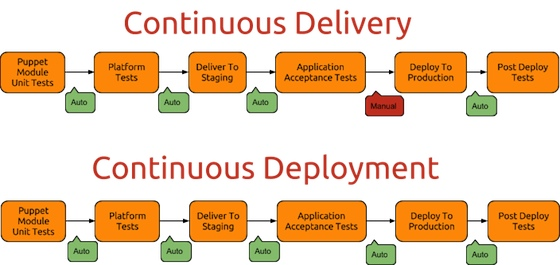
\includegraphics[width=\textwidth,height=\textheight,keepaspectratio]{Introduction/Continuous_Delivery_Continuous_Deployment.jpg}
\caption{Continuous delivery and continuous deployment pipelines}
\end{figure}

The infrastructure requirements for continuous deployment are higher than
the previous ones because we should be able to deploy automatically after
a working change and roll back in case of problems. Any change is tested
with automatic tests and if the tests fail the deployment should abort. On
the other hand, if the version deployed is broken, because the tests did
not detect the problem, then the team needs to be able to roll back and
fix the problem.
